Neste capítulo, será apresentado inicialmente definições do domínio do problema de classificação e identificação de cenas em sensoriamento remoto na seção~\ref{sec:Cap2_dominio}, bem como suas características e contexto. Seguindo por um apanhado teórico da seção envolvendo aprendizado de máquina, redes neurais, redes neurais profundas, convolucionais e~\textit{transformers}, no que tange interseções com possíveis soluções para o problema.
E por fim, na seção~\ref{sec:Cap2_revisao_literatura} uma revisão da literatura e do atual estado da arte no que tange o problema de classificação visual no que tange a sensoriamento remoto. Apresentando trabalhos que envolveram soluções tanto para o campo, quanto para implementações de redes neurais profundas.


% trabalhos:
% -\textit{transformers}pra label da amazonia
% - Unet pra detecção de garimpo,
% - attention is all you need,
% - a image worth 16x16,
% - paper principal da cnn Alexnet,
% - solução desse problema via cnn.

\section{\textit{Domínio do problema}}\label{sec:Cap2_dominio}
% TODO: fonte definição sensoriamento remoto
\begin{figure}[!ht]
    \centering
    \includegraphics[width=0.9\columnwidth]{
        Imagens/instrutorgis\_sensoriamento\_remoto\_ilustracao.png
    }
    \caption{Sensoriamento remoto Foto:\cite{InstrutorGIS}}
\label{fig:sensoriamento}
\end{figure}

O problema em questão, de identificação de regiões com garimpo em imagens de satélite, e pertencem ao campo de sensoriamento remoto. O sensoriamento remoto consiste em aquistar ou analisar medições de uma região geográfica terrestre, ou atmosférica. Podem ser realizadas por imagens aéreas ou por satélites, podendo abranger diferentes partes do espectro eletromagnético.
Frequentemente consistem em métodos de aquisição ou processamento de sinais e imagens, para obter características ou reconhecer padrões em tais localidades~\cite{emery2017introduction}.O termo foi cunhado referir-se a medição realizada por algum meio indireto ou “remoto”, em vez de um contato direto com sensores no ambiente medido~\cite{emery2017introduction}.


Ainda mais especificamente, o problema introduzido também faz parte do campo de reconhecimento de padrões em imagens. Temos que a área varrida por sensoriamento remoto é extensiva para ser vasculhada manualmente. Portanto, se faz necessário o uso de algorítimos que automatizem a detecção ou classificação do objeto a ser encontrado.
O campo de reconhecimento de padrões possui algorítimos tradicionais para identificar e localizar objetos de interesse, porém podem ser muito caras computacionalmente e pouco efetivas, dependendo das características do problema. Por isso, tem recentemente sido frequentemente empregadas técnicas baseadas em aprendizado de máquina e aprendizado profundo, que atualmente são o estado da arte em muitos problemas de reconhecimento de padrões.


\section{Revisão Teórica}\label{sec:Cap2_revisao_teorica}

\subsection{Aprendizado de máquina}\label{sec:aprendizado_maquina}

Aprendizado de máquina é um campo que estuda algorítimos capazes de aprender e realizar inferências a partir de dados. O termo foi cunhado em 1959, por Artur Samuel, como “Campo de estudos que visa a dar computadores a habilidade de aprender sem serem explicitamente programados para determinada tarefa.”~\cite{Samuel1959SomeSI}.

Já em~\cite{Mitchell97} define um algorítimo de aprendizado como “Um algoritmo dito conseguir uma experiência E com respeito a determinada classe de tarefas T e com medidas de desempenho P, se seu desempenho nas tarefas em T, medidas por P, melhoram a partir da experiência E.”

Para melhor entender cada constituinte dessa definição, podemos utilizar de um exemplo. A tarefa T temos como exemplo o problema de classificação, que consiste do algorítimo responder quais das k categorias para o qual ele experimentou em E, certas amostras de entradas pertencem. Para resolver tal tarefa, tal algorítimo de aprendizado deve produzir uma função \(f:\Re^n\rightarrow \{1,\ldots,k\}\). Quando \( y=f(x) \), o modelo atribui uma entrada descrita pelo por \(x\), que nosso caso constitui uma amostra de entrada, a uma categoria identificada por um código numérico \(y\). Uma variante do mesmo problema é em vez de classificar qual classe, retornar a distribuição de probabilidade sobre as classes~\cite{GoodBengCour16}. A medida de desempenho P, necessária para avaliar as habilidades de um dado algorítimo. Tal medida de desempenho é geralmente atrelada ao tipo de tarefa sendo realizada pelo sistema. 

\subsection{Métricas de desempenho}\label{sec:cap2_metricas_desempenho}


Para tarefas de classificação, é comumente utilizada a métrica de acurácia do modelo. Consiste na proporção de amostras na qual o modelo produz a saída correta. Sejam verdadeiros positivos $vp$, falsos positivos $fp$, verdadeiros negativos $vn$, falsos negativos $fn$, temos que a acurácia AC é:
\begin{equation}AC = \frac{tp + tn}{tp + tn + fp + fn} \end{equation}

\begin{itemize}
    \item Verdadeiros Positivos: classificação correta da classe Positivo
    \item Falsos Positivos (Erro Tipo I): erro onde o modelo previu a classe Positivo quando o rótulo era classe Negativo
    \item Falsos Negativos (Erro Tipo II): erro onde o modelo previu a classe Negativo quando o rótulo era classe Positivo
    \item Verdadeiros Negativos: classificação correta da classe Negativo
\end{itemize}

Cada uma dessas métricas são representadas na chamada matriz confusão, como ilustra a figura \ref{fig:metricas}.

Para problemas de multiclasses e multirótulos, ainda temos a métrica acurácia até o n-ésimo candidato, denotado por AC@n. Por exemplo: AC@5 é acurácia do verdadeiro positivo estar dentre os primeiros 5 candidatos sugeridos.

Outras métricas também podem ser interessantes em casos onde amostras das classes são muito desbalanceadas, métricas $F_\beta$ e curva precisão-revocação. Sejam Precisão $P$ e revocação $R$, temos que:



\begin{figure}[!ht]
    \centering
    \begin{minipage}[c]{0.4\textwidth}
        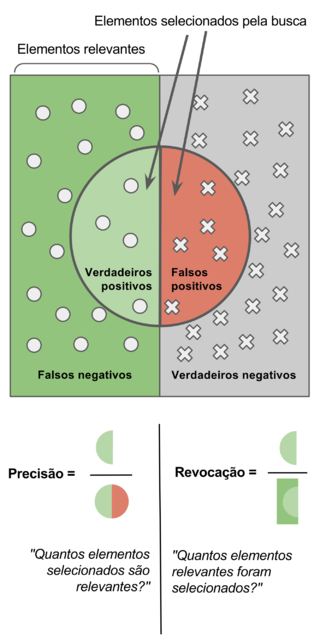
\includegraphics[width=\columnwidth]{Imagens/Precisão_e_revocação.png}
        \caption{Ilustração das métricas de precisão e revocação.}
    \end{minipage}%
    \begin{minipage}{0.5\textwidth}
        \includegraphics[width=\columnwidth]{Imagens/matrix_confusão.png}
        \begin{equation} P = \frac{vp}{vp + vp} \end{equation}
        \begin{equation}R = \frac{vp}{vp + fp}\end{equation}
        \begin{equation}F_\beta = (1+\beta^2) \times \frac {P \times R}{\beta^2 P + R}\end{equation}
        \begin{equation}F_2 = 5 \times \frac {P \times R}{5 P + R}\end{equation}
        \caption{Matriz Confusão, Equações de Precisão, revocação, $F_\beta$ e $F_2$}        
    \end{minipage}       
    \label{fig:metricas}
\end{figure}

Altas taxas de precisão e revocação mostram que o classificador está retornando resultados relevantes, com poucos falsos positivos (Precisão) e também retornando a maioria de todos os resultados positivos (Revocação) \cite{hastie01statisticallearning}. Um sistema com alta revocação e baixa precisão retorna muitos resultados, mas muitos deles incorretos, enquanto um com alta precisão e baixa revocação retorna na maioria corretos, mas poucos resultados.

A métrica $F_\beta$ é uma média harmônica entre precisão e revocação, portanto sumariza o compromisso entre esses dois índices  e pesa a importância de cada a partir de $\beta$.

Podemos comparar métricas e modelos a partir do chamado classificador ingênuo, que atribui a probabilidade de uma classe ser positiva apenas pela frequência de positivos de tal classe no conjunto de dados:

\begin{equation}
    ProbClassIng(X|y=1) = \frac{P}{P + N}
\end{equation}

Em um conjunto de dados muito desbalanceado, métrica de acurácia é pouco capaz de refletir o quão a desempenho de um modelo é superior ao classificador ingênuo, pois possuem acurácias próximas. Enquanto Precisão-Revocação e métrica $F_2$ consegue melhor diferenciar do classificador ingênuo e é capaz de avaliar o índice de revocação.

Um classificador que retorna a probabilidade de pertencimento de cada classe pode classificar tal classe como positiva ou não ao se comparar com determinado limiar.

A curva precisão-revocação ilustra a relação de compromisso entre os dois índices para diferentes limiares. Uma área grande abaixo da curva representa ambos alta precisão e revocação para muitos limiares diferentes. Do contrário, uma área abaixo da curva \footnote[1]{Area under the curve - AUC} representa que independente do limiar escolhido para o classificador, apresentará baixa precisão e revocação.

Outra métrica para avaliação de classificadores é a curva COR \footnote[2]{Comumente chamada de ROC - Receive Operator Characteristic}, contudo apresenta resultados otimistas para conjuntos de dados balanceados, assim como a acurácia.

Para ambas curvas PR e ROC, um modelo é qualitativamente bom quanto mais desempenho tiver em comparação com o classificador ingênuo, que escolhe classifica com a probabilidade da frequência daquela classe ou aleatoriamente.

\subsection{Função de perda}\label{sec:cap2_fucao_de_perda}

Como métricas de perda para tarefas de classificação, podem ser utilizadas, por exemplo, a entropia cruzada, dada por:

Otimizadores possuem como objetivo ajustar pesos de uma função de custo para minimizar ou maximizar tal custo. Para quantificar o custo são utilizadas métricas de perda. Dentre elas, as funções de custos ideais para classificação binária multiclasses e multirótulos temos a entropia binária cruzada, definida por 
$$ECB(y_c) = -\sum_{c=0}^{M} y_c \times log(\hat{y_c})$$
sendo $p(\hat{y_c})$ a probabilidade. 

Para conjuntos de dados muito desbalanceados, pode-se mitigar o sobre-ajuste da classe dominante utilizando BCE com pesos do inverso da frequência das classes:
$$ C_i = \frac{FN}{VP_i} $$
$$ECB(y_c) = -\sum_{c=0}^{M} C_i \times y_c \times log(\hat{y_c})$$


Outra solução para mitigar o mesmo problema é a função de perda focal. Consiste em uma ECB penalizando exponencialmente por um peso gama as classificações com probabilidades altas.\cite{https://doi.org/10.48550/arxiv.2106.10270}

$$Focal(y_c) = -\sum_{c=0}^{M} (1-w_i \times y_c)^\gamma \times log(\hat{y_c})$$

\subsection{Redes Neurais Artificiais}\label{sec:Cap2_redes_neurais}

O termo redes neurais embarca uma grande classe de modelos e métodos de aprendizados. O modelo mais simples, também podendo ser chamado rede de camada oculta única de perceptrons. Já o  perceptron é a célula de uma rede neural. Se trata de um modelo matemático análogo a um neurônio. Possui um vetor de entradas e sobre essas entradas é aplicada uma combinação linear utilizando os pesos sobre cada entrada. O resultado de tal operação por sua vez passa por uma função de ativação que resulta numa saída binária de classificação do perceptron. Dessa forma, ao se otimizar os pesos e função de ativação a determinadas amostras de treino e suas respectivas saídas rotuladas, podemos criar um classificador linear simples, caso seja um problema linearmente separável. Portanto, o processo de treinamento de uma rede neural se trata de otimizar os pesos dos neurônios. 
Uma etapa importante dos ajustes dos pesos é a retro-propagação de erro\footnote{Frequentemente citada como \textit{Backpropagation}} a qual é um algoritmo que otimiza os pesos da camada oculta~\cite{hastie01statisticallearning}. 

Para classificações multiclasses e multirótulos, isto é, uma amostra pode pertencer a mais de uma classe simultaneamente, são utilizadas camadas de saída que implementam normalização para selecionar a probabilidade de cada classe. Temos como exemplo a camada de ativação \textit{Sigmoid} \ref{fig:sigmoid}. 
Pode ser interpretada como probabilidade, portanto $\sigma(z(x))$ é a probabilidade de X pertencer à classe positiva e $1-\sigma(z(x))$ a de não pertencer à classe positiva.

\begin{figure}[!ht]
    \centering
    \begin{minipage}[c]{0.4\textwidth}
        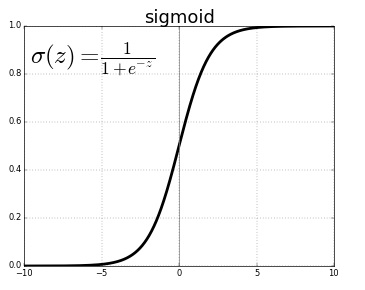
\includegraphics[width=\columnwidth]{Imagens/sigmoid-activation-function.jpg}
        \caption{Função de ativação \textit{Sigmoid}.}
    \end{minipage}%
    \begin{minipage}{0.5\textwidth}
        \begin{equation} Sigmoid(x) = \sigma(x) = \frac{1} {1+ exp(-x)}\end{equation}
    \end{minipage}       
    \label{fig:sigmoid}
\end{figure}


\begin{figure}[!ht]
    \centering
        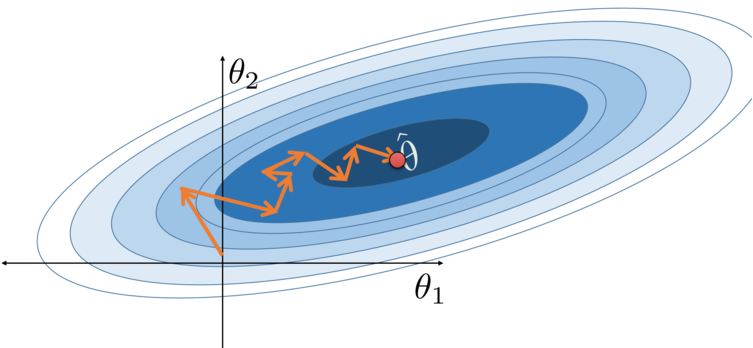
\includegraphics[width=0.47\columnwidth]{Imagens/stochastic_gradient_descent.PNG}
    \caption{Exemplo de algorítimo de otimização: gradiente descendente estocástico. }
    \label{fig:SGD}
\end{figure}






\begin{figure}[!ht]
    \centering
    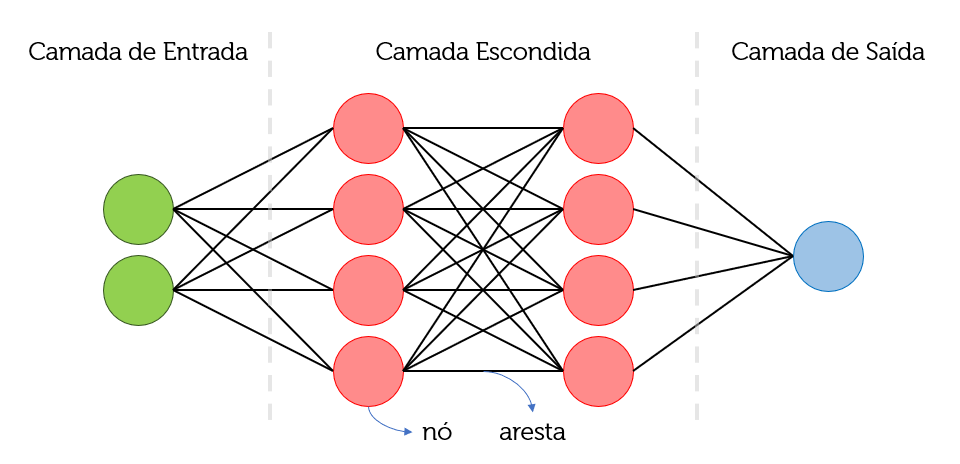
\includegraphics[width=0.6\columnwidth]{
        Imagens/RedeNeural.PNG
    }
    \caption{Exemplo de uma rede de perceptrons de multiplas camadas - MLP.}
    \label{fig:ann}
\end{figure}
\subsection{Redes Neurais Artificiais Profundas}\label{sec:Cap2_redes_neurais_profundas}
O termo redes neurais profundas e o aprendizado profundo, ou comumente chamado de \textit{deep learning}, se refere a redes neurais artificiais com múltiplas camadas ocultas. Foram uma das tecnologias maior desenvolvidas nos últimos anos, e se tornaram cada vez mais popular. Devido a sua superior \textit{performance} em extração de características, teve sucesso por distintos domínios, como visão computacional, reconhecimento de fala, processamento natural de linguagem e em big data.

Um dos riscos envolvendo o treinamento de redes neurais profundas é o problema de \textit{overfiting}\footnote{Sobre-ajuste}. Se trata de quando o modelo é treinado e para gerar uma função próxima demais aos dados de treino, e perdem generalidade, falhando em predições em dados fora do conjunto de treino. Para mitigar o surgimento de \textit{overfiting} durante o treino, são utilizadas técnicas de regularização. Consistem em adicionar penalidade à complexidade do modelo, de forma que o treino otimize para se tornar uma função genérica. Dentre as técnicas de regularização possíveis de DNNs\footnote{\textit{Deep Neural Networks}}, podemos citar o \textit{Dropout, Dropconnect e pruning}, que consistem em respectivamente a remoção, adição de conexão entre neurônios e remoção de neurônios~\cite{hastie01statisticallearning}.


\subsection{Redes Neurais Convolucionais}\label{sec:Cap2_redes_neurais_convolucionais}
Uma arquitetura clássica é a rede neural convolucional (CNN\footnote{\textit{Convolutional Neural Network}}), que utiliza convoluções para extrair características de uma imagem entre cada camada de filtros. Também possui camadas de \textit{pooling}, não lineares e camadas completamente conectadas~\cite{8308186}. Uma dos pressupostos das \textit{CNNs} é os filtros serem indiferentes a translações das características na imagem, possibilitando assim uma eficiente extração de características para composição e identificação da imagem.


Em 2012, o modelo de CNN AlexNet ultrapassou em desempenho os modelos do estado da arte em uma grande margem. Dois fatores promoveram tal degrau de evolução: a disponibilidade de grandes \textit{datasets}\footnote{Conjunto de dados} como o ImageNet e a comoditização de placas gráficas, que promoveram significativamente mais poder computacional para treino, já que são aceleradores de operações vetorizadas e sobre matrizes. Dessa forma, desde 2012 CNNs se tornaram o modelo padrão para tarefas de visão computacional \cite{alom2018history}.

A maior vantagem dos modelos CNN em comparação com os métodos anteriores era de conseguir ser treinados ponta a ponta, sem a necessidade de criação de filtros ou a criação manual de extratores de características visuais. Também possuem duas importantes propriedades como invariância translacional, isto é, o sistema produz a mesma resposta independente de translação; e campo receptivo restrito, o que significa que neurônios das primeiras camadas capturam detalhes finos e locais.
\begin{figure}[!ht]
    \centering
    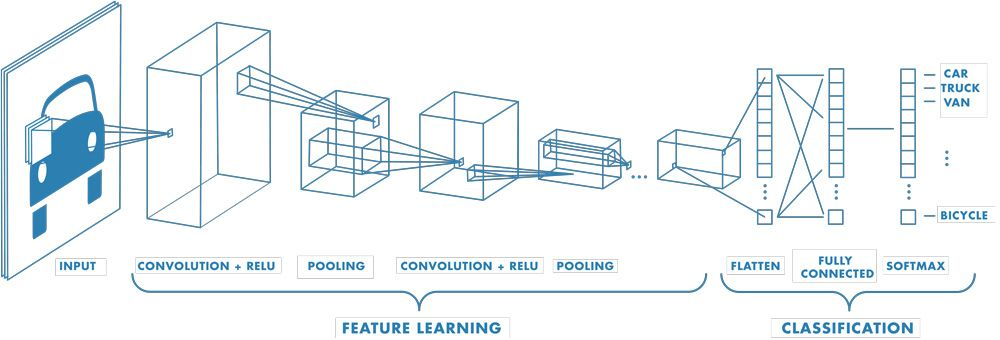
\includegraphics[width=0.95\columnwidth]{
        Imagens/CNN_mathworks.jpg
    }
    \caption{Arquitetura de uma rede convolucional. Filtros extratores de características são aplicados em diferentes resoluções e campos visuais. A saída de cada imagem convoluta alimenta a próxima camada. As últimas camadas completamente conectadas realizam a classificação.}
    \label{fig:cnn}
\end{figure}

\begin{figure}[!ht]
    \centering
    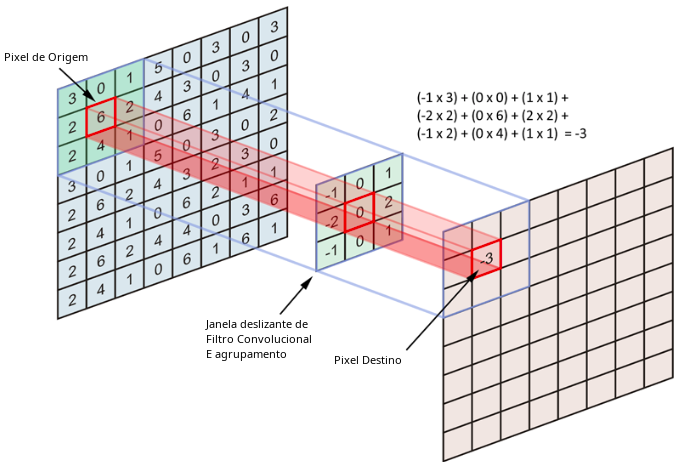
\includegraphics[width=0.6\columnwidth]{
        Imagens/operacao_conv.png
    }
    \caption{
 Filtro convolucional que aplica uma janela deslizante aplicando operação de convolução e pooling.  
        % --- Source: https://towardsdatascience.com/applied-deep-learning-part-4-convolutional-neural-networks-584bc134c1e2
    }
    \label{fig:conv}
\end{figure}

\subsection{\textit{ResNet}}\label{sec:Cap2_ResNet}

Após a primeira arquitetura AlexNet, a arquitetura subsequentes utilizaram mais camadas em uma rede neural profunda para gerar melhores modelos. Contudo, sofreram de um problema de convergência de otimização e regularização, chamado explosão de gradiente. Consiste no fato de quando o número de camadas é muito alta há gera gradientes muito altos ou se tornam zero, fazendo com que o treinamento não tenha convergência. 
Para solucionar este problema, foi proposta a arquitetura de redes residuais, que possuem conexões saltos, conectando camadas de diferentes profundidades, como ilustra \ref{fig:ResNet-Rsp}. Possibilitando a propagação de gradiente saltando camadas. Assim mitigou o problema de explosão de gradientes e permitiu, desde então, a escalabilidade de redes neurais profundas. 


\begin{figure}[!ht]
    \centering
    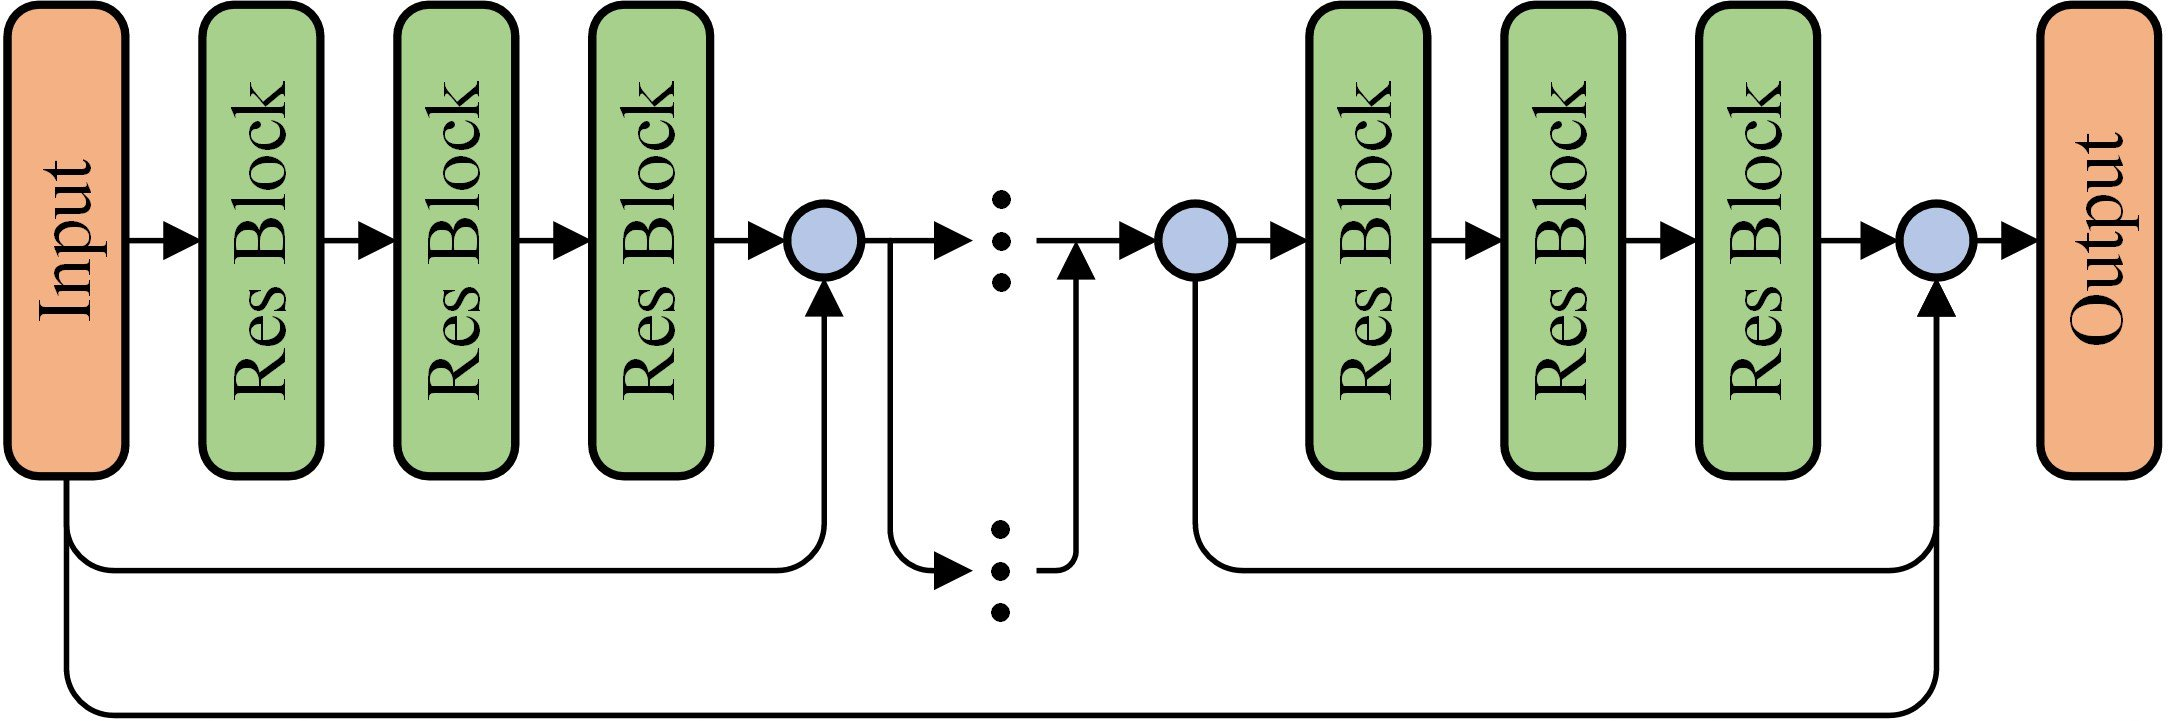
\includegraphics[width=0.9\columnwidth]{Imagens/An-illustration-of-the-deep-residual-network-ResNet-structure-More-shortcut.jpg}
    \caption{ Arquitetura de modelo base. Fonte:WikiCommons}
   \label{fig:ResNet-Rsp}
\end{figure}


\subsection{\textit{O problema de rotulagem e variabilidade de amostras de treino}}\label{sec:Cap2_rotulagem}

Um dos principais desafios envolvido o treino de \textit{CNNs} aplicado a sensoriamento remoto é representar um estado de características que cubram as variações fotográficas, tanto em características do sensor, como variações da imagem no dia, clima, estação e plataforma da câmera, o que se torna uma tarefa difícil. Para uma localização efetiva, o modelo deve ser robusto a todas essas variações, que requer um grande conjunto de treino que cobre boa parte das diversas condições possíveis. Tal conjunto de dados não é disponível e nem viável de obter, pois se trata um volume muito grande de amostras. Tais limitações levam a necessitar o desenvolvimento de algorítimos que aprendem seletivamente para que o poder computacional seja utilizado eficientemente, bem como reutilizar conhecimento prévio e evitar treinamento redundante~\cite{rostami2019learning}.  Dentre as técnicas utilizadas para implementar esses modelos mais eficientes, temos como exemplo o aprendizado supervisionado fraco, e a transferência de aprendizado.

\subsection{\textit{Aprendizado semi-supervisionado}}\label{sec:Cap2_semisup}

As técnicas de aprendizado semi-supervisionado consistem em treinar um modelo com apenas um conjunto reduzido de amostras rotuladas de treino, e as demais amostras serem não supervisionadas. As demais amostras de treino podem ser utilizadas, por exemplo, agrupando-as com as amostras rotuladas e classificando-as como a amostra mais próxima, como apresenta o trabalho de~\cite{Sanches2003}. Outras propostas envolvem~\textit{data augmentation}\footnote{Aumento de dados}, que consistem em gerar um conjunto de treino maior, dados as amostras de treino disponíveis.

\subsection{\textit{Transferência de aprendizado}}\label{sec:Cap2_transfer}

Já técnicas de transferência de aprendizado\footnote{Comumente citado como Transfer Learning}, ou \textit{few shots learning}, consistem em redes treinadas para um conjunto limitado de testes~\cite{rostami2019learning}
e reutilizam esse conhecimento através de diferentes domínios, tarefas ou agentes. Consistem primariamente de um problema origem e um problema objetivo e como podemos suceder em transferir conhecimento dado o problema origem. A abordagem de transferência de conhecimento se inspira em replicar a habilidade humana em que é possível transferir conhecimento de experiências passadas para lidar com tarefas com poucas amostras rotuladas. Este fato inspirou em representar dados de diferentes problemas de aprendizado de máquina em um espaço embutido onde as representações utilizam de diversas relações entre diferentes domínios de conhecimentos e tarefas. Uma implementação encontrada na literatura, proposta em~\cite{rostami2019learning}, consistiu de transplantar a camada de características de uma CNN derivada do domínio de origem para inicializar outra rede, do domínio objetivo, composta por uma camada final fortemente conectada. Assim foi aproveitada as primeiras camadas e a rede foi trenada para o domínio objetivo com uma quantidade menor de amostras.


\section{Transformer Visual}\label{sec:Cap2_transformer_visual}


Temos que a arquitetura de CNNs em si, é projetada especificamente para imagens e podem ser computacionalmente onerosas, dessa forma podendo não escalar ou generalizar o suficiente para modelos multimodais. Diante dessas limitações, foram pesquisados modelos que possam escalar e serem agnósticos em quesito de domínios de aplicação. Nessa direção que em \cite{dosovitskiy2020image} é criado o\textit{Transformer} Visual ou ViT \footnote{\textit{Vision Transformer}}, uma arquitetura modelo de visão baseado na possibilidade da utilização da arquitetura Transformer, originalmente utilizada para tarefas baseadas em texto, para tarefas de visão computacional.

O ViT representa uma imagem de entrada como uma sequência de recortes de imagem, similarmente a uma sequência de representações de palavras quando aplicado Transformers para texto, e diretamente predizendo a classe de rótulo da imagem. Tal arquitetura e suas variações apresentaram excelente desempenho, superando a de CNNs até então estado-da-arte, a ResNet, consumindo até um quarto de recursos computacionais.


O\textit{transformer}original recebe como entrada uma sequência de palavras, que então usa para classificação, tradução ou outras tarefas de processamento natural de linguagem. Para o ViT, em \cite{dosovitskiy2020image} foram aplicadas poucas modificações, para mesma arquitetura ser aplicada a imagens em vez de palavras, e assim observar como o modelo aprende por si próprio.

\begin{figure}[!ht]
    \centering
    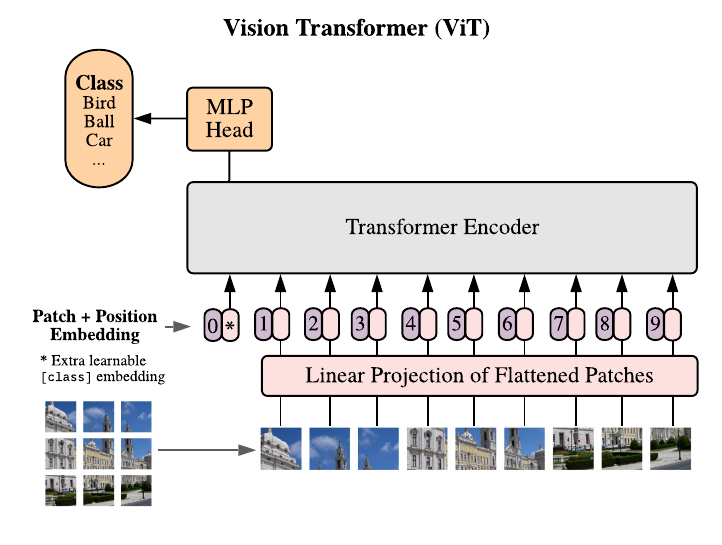
\includegraphics[width=0.65\columnwidth]{
        Imagens/vit.png
    }
    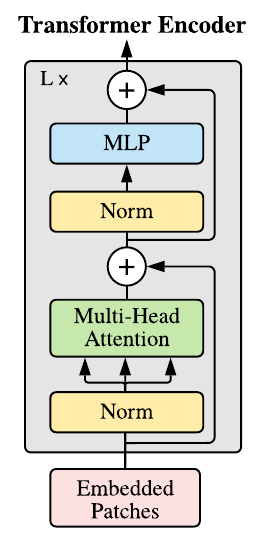
\includegraphics[width=0.34\columnwidth]{
        Imagens/encoder.png
    }
    \caption{O ViT divide uma imagem em uma grade de recortes quadrados, cada fragmento é achatado em um vetor único contendo todos os canais de todos os pixeis, e projetando-os em uma dimensão de entrada desejada, alimentando a camada de múltiplos Encoders em paralelo. \cite{dosovitskiy2020image}}
    \label{fig:vit}
\end{figure}


\subsection{\textit{Arquitetura do \textit{transformer} visual}}\label{sec:Cap2_vit}

% Mecanismo de atenção
% 

O \textit{encoder do transformer} é composto por:
\begin{itemize}
    \item Camada de múltiplas cabeças de atenção (MSP): Esta camada concatena todas as saídas de atenção linearmente para a dimensão correta. As várias cabeças de atenção ajudam a treinar local e globalmente dependências em uma imagem.
    \item Camada de múltiplas (MLP) camadas de perceptrons: contem um MLP de duas camadas com função de ativação GELU (Unidade de erro linear Gaussiano)
    \item Camada de normalização (LN): Adicionada antes de cada bloco e normaliza os pesos dentro de uma mesma camada.
    \item Saltos de conexão: somam a saída de blocos a entrada. Desempenha papel de auxiliar a convergência da otimização do gradiente descendente e explosão de gradientes.
\end{itemize}

A MSP é o núcleo do \textit{encoder}\footnote{Codificador} implementa o mecanismo de autoatenção. Consiste em relacionar diferentes posições de uma única sequência para se computar uma representação desta sequência \cite{AttentionIsAllYouNeed}.

%\begin{figure}[!ht]
%    \centering
%    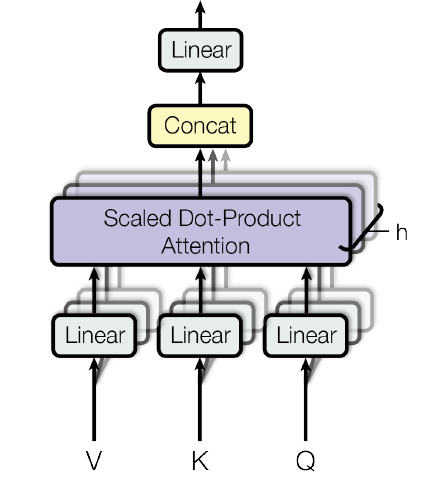
\includegraphics[width=0.4\columnwidth]{
%        Imagens/Multi-Head Attention.png
%    }
%    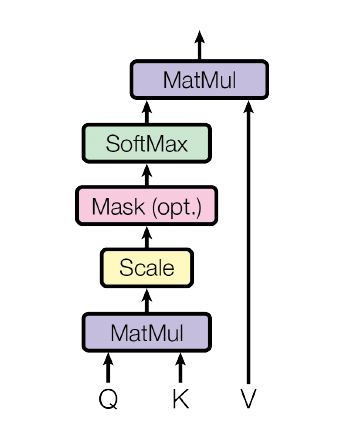
\includegraphics[width=0.4\columnwidth]{
%        Imagens/Scaled Dot-Product Attention.png
%    }
%    \caption{Exemplo de uma rede convolucional. Filtros são aplicados em diferentes resoluções. A saida de cada imagem convoluída alimenta a próxima camada.}
%    \label{fig:attention}
%\end{figure}

% https://towardsdatascience.com/transformers-explained-visually-part-3-multi-head-attention-deep-dive-1c1ff1024853



\begin{figure}[!ht]
    \centering
    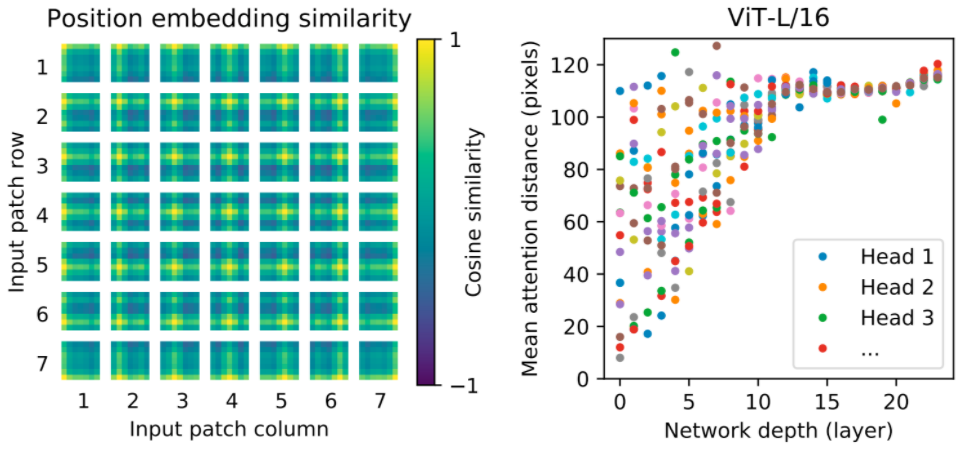
\includegraphics[width=0.9\columnwidth]{
        Imagens/ViTVisualization.png
    }
    \caption{
        Esquerda: ViT aprende a estrutura de grade via representações de posição. Direita: Camadas inferiores do ViT contem ambas características locais e globais, o quão mais profundas as camadas, mais globais as características.\cite{dosovitskiy2020image}
        }
    \label{fig:ViTVisualization}
\end{figure}


É possível observar como o modelo aprende ao visualizar alguns comportamentos internos. Ao observar as representações de posição, os parâmetros do modelo que aprendem a codificar a representação relativa dos recortes, encontramos que o ViT consegue reproduzir intuitivamente uma estrutura de imagem. Cada representação de posição é mais similar a outras da mesma coluna e linha, indicando que o modelo recuperou a estrutura de grade das imagens originais. Em segundo lugar, examinando a distância espacial médio entre elementos para cada bloco \textit{transformer}. Em camadas mais profundas, apenas características globais são utilizadas, ou seja, grandes distâncias de atenção. Enquanto camadas mais rasas capturam ambas características globais e locais, indicado por uma faixa grande de atenção. Em contraste, apenas características locais são presentes nas camadas superficiais das CNNs. Estes experimentos indicam que ViT aprendem características codificadas manualmente nas CNNs, como percepção da estrutura de grade. E principalmente revela que tais modelos são livres para aprender padrões mais genéricos, como mistura de características globais e locais, dessa forma contribuindo para generalização~\cite{dosovitskiy2020image}.
 

\begin{figure}[!ht]
    \centering
    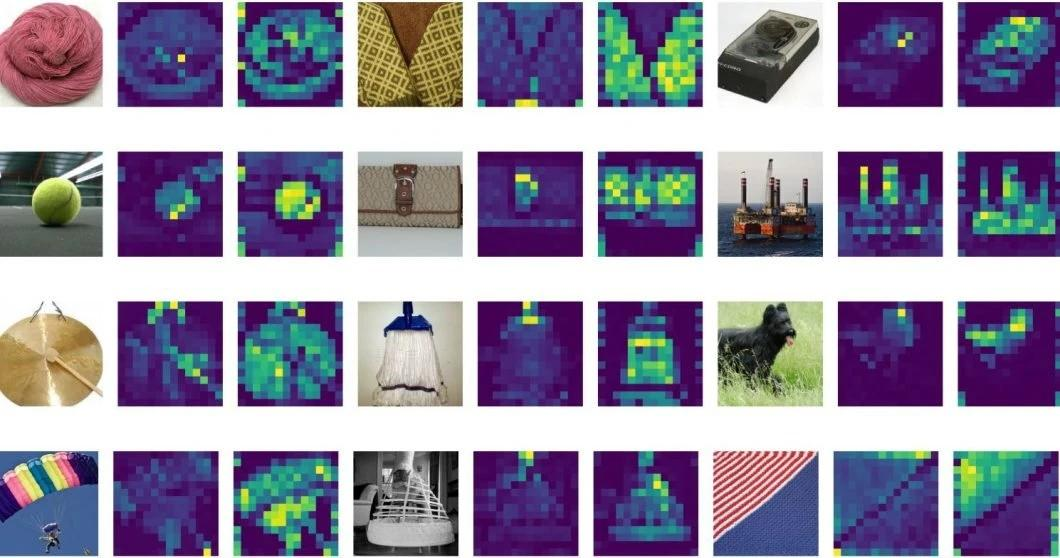
\includegraphics[width=\columnwidth]{
        Imagens/visualizing-attention-vit.jpg
    }
    \caption{
O modelo lida com as regiões que são semanticamente relevantes para classificação. \cite{ViTvsResNets}
        }
    \label{fig:ViTVisualizationAttention}
\end{figure}



\section{Trabalhos anteriores}\label{sec:Cap2_revisao_literatura}

\subsection{Problema de detecção de mudanças em minas de menor escala}\label{sec:Cap2_deteccao_mudanca}

Em \cite{rs14071746} foi gerado um \textit{dataset}\footnote{Conjunto de dados} para detecção de mudanças e de mineração de ouro em menor escala. Com os dados rotulados, foram testadas abordagens supervisionadas e semi-supervisionadas e extratores de características para encontrar um melhor modelo detector de mudanças. Obtiveram o melhor modelo baseado no método E-ReCNN, utilizando seis canais e treino supervisionado, com pontuação f1 de $0.88\pm0.05$.

\subsection{Classificação de minas e represas}\label{sec:Cap2_minas_represa_classificacao}

O problema de classificação para detecção em sensoriamento remoto, utilizando aprendizado profundo, foi explorado em ~\cite{s20236936}, utilizando imagens multiespectrais do satélite \textit{Sentinel-2}. Consistiu em treinar um modelo baseado em CNN para identificar em recortes da imagem qual classe pertence.

\subsection{Pré-treino de \textit{transformers} visuais para sensoriamento remoto}\label{sec:Cap2_million}

Para a aplicação de sensoriamento remoto temos trabalhos~\cite{wang2022empirical} que demonstram a aplicação de transferência de aprendizado e redes pré-treinadas utilizando ViT estado-da-arte. Utilizou-se o \textit{dataset} MillionAID, o maior \textit{dataset} datado até agora para sensoriamento remoto. Contem mais de um milhão de imagens sem sobreposição, com múltiplas visões temporais para a mesma cena, de canais apenas RGB. Possui uma árvore de classificação com 51 folhas, de cenas de terras de: agricultura, comercial, industrial, serviço público, industrial, transporte, regiões com água e regiões inutilizadas. Cada Folha possui 2.000~45,000 imagens. Foram obtidas pelo \textit{software Google Earth}, que possui uma diversidade de sensores, resultando em diferentes resoluções, desde 50 cm à 150 m. E tamanhos de imagem de 10k pixeis até 900 mega pixeis.
O autor pode concluir que a transferência de aprendizado foi eficaz para posteriores finetune\footnote{Ajuste fino.}.

\subsection{Transformer Swin}\label{sec:Cap2_Swin}

Em~\cite{liu2022swin} foi proposto uma arquitetura de transformer visual com melhorias capazes de reduzir o custo computacional do cálculo de atenção entre cada recorte da imagem de entrada. Este trabalho aponta que a ordem de complexidade do ViT clássico é $O(n^2)$, sendo $n$ o número de retalhos, já que é calculado a métrica de atenção entre cada retalho com todos os outros demais. Com isso, torna caro o treino para maiores resoluções ou granularidade de detalhes. A arquitetura Swin, ou \textit{Shifted Window} se baseia em uma disposição hierárquica de Transformers, como ilustra a figura \ref{fig:SWIN-arquitetura}, sendo que nas camadas mais baixas, coletam atenção apenas localmente e não com todo restante da imagem. Dessa forma o custo se torna aproximadamente linear. 


\begin{figure}[!ht]
    \centering
    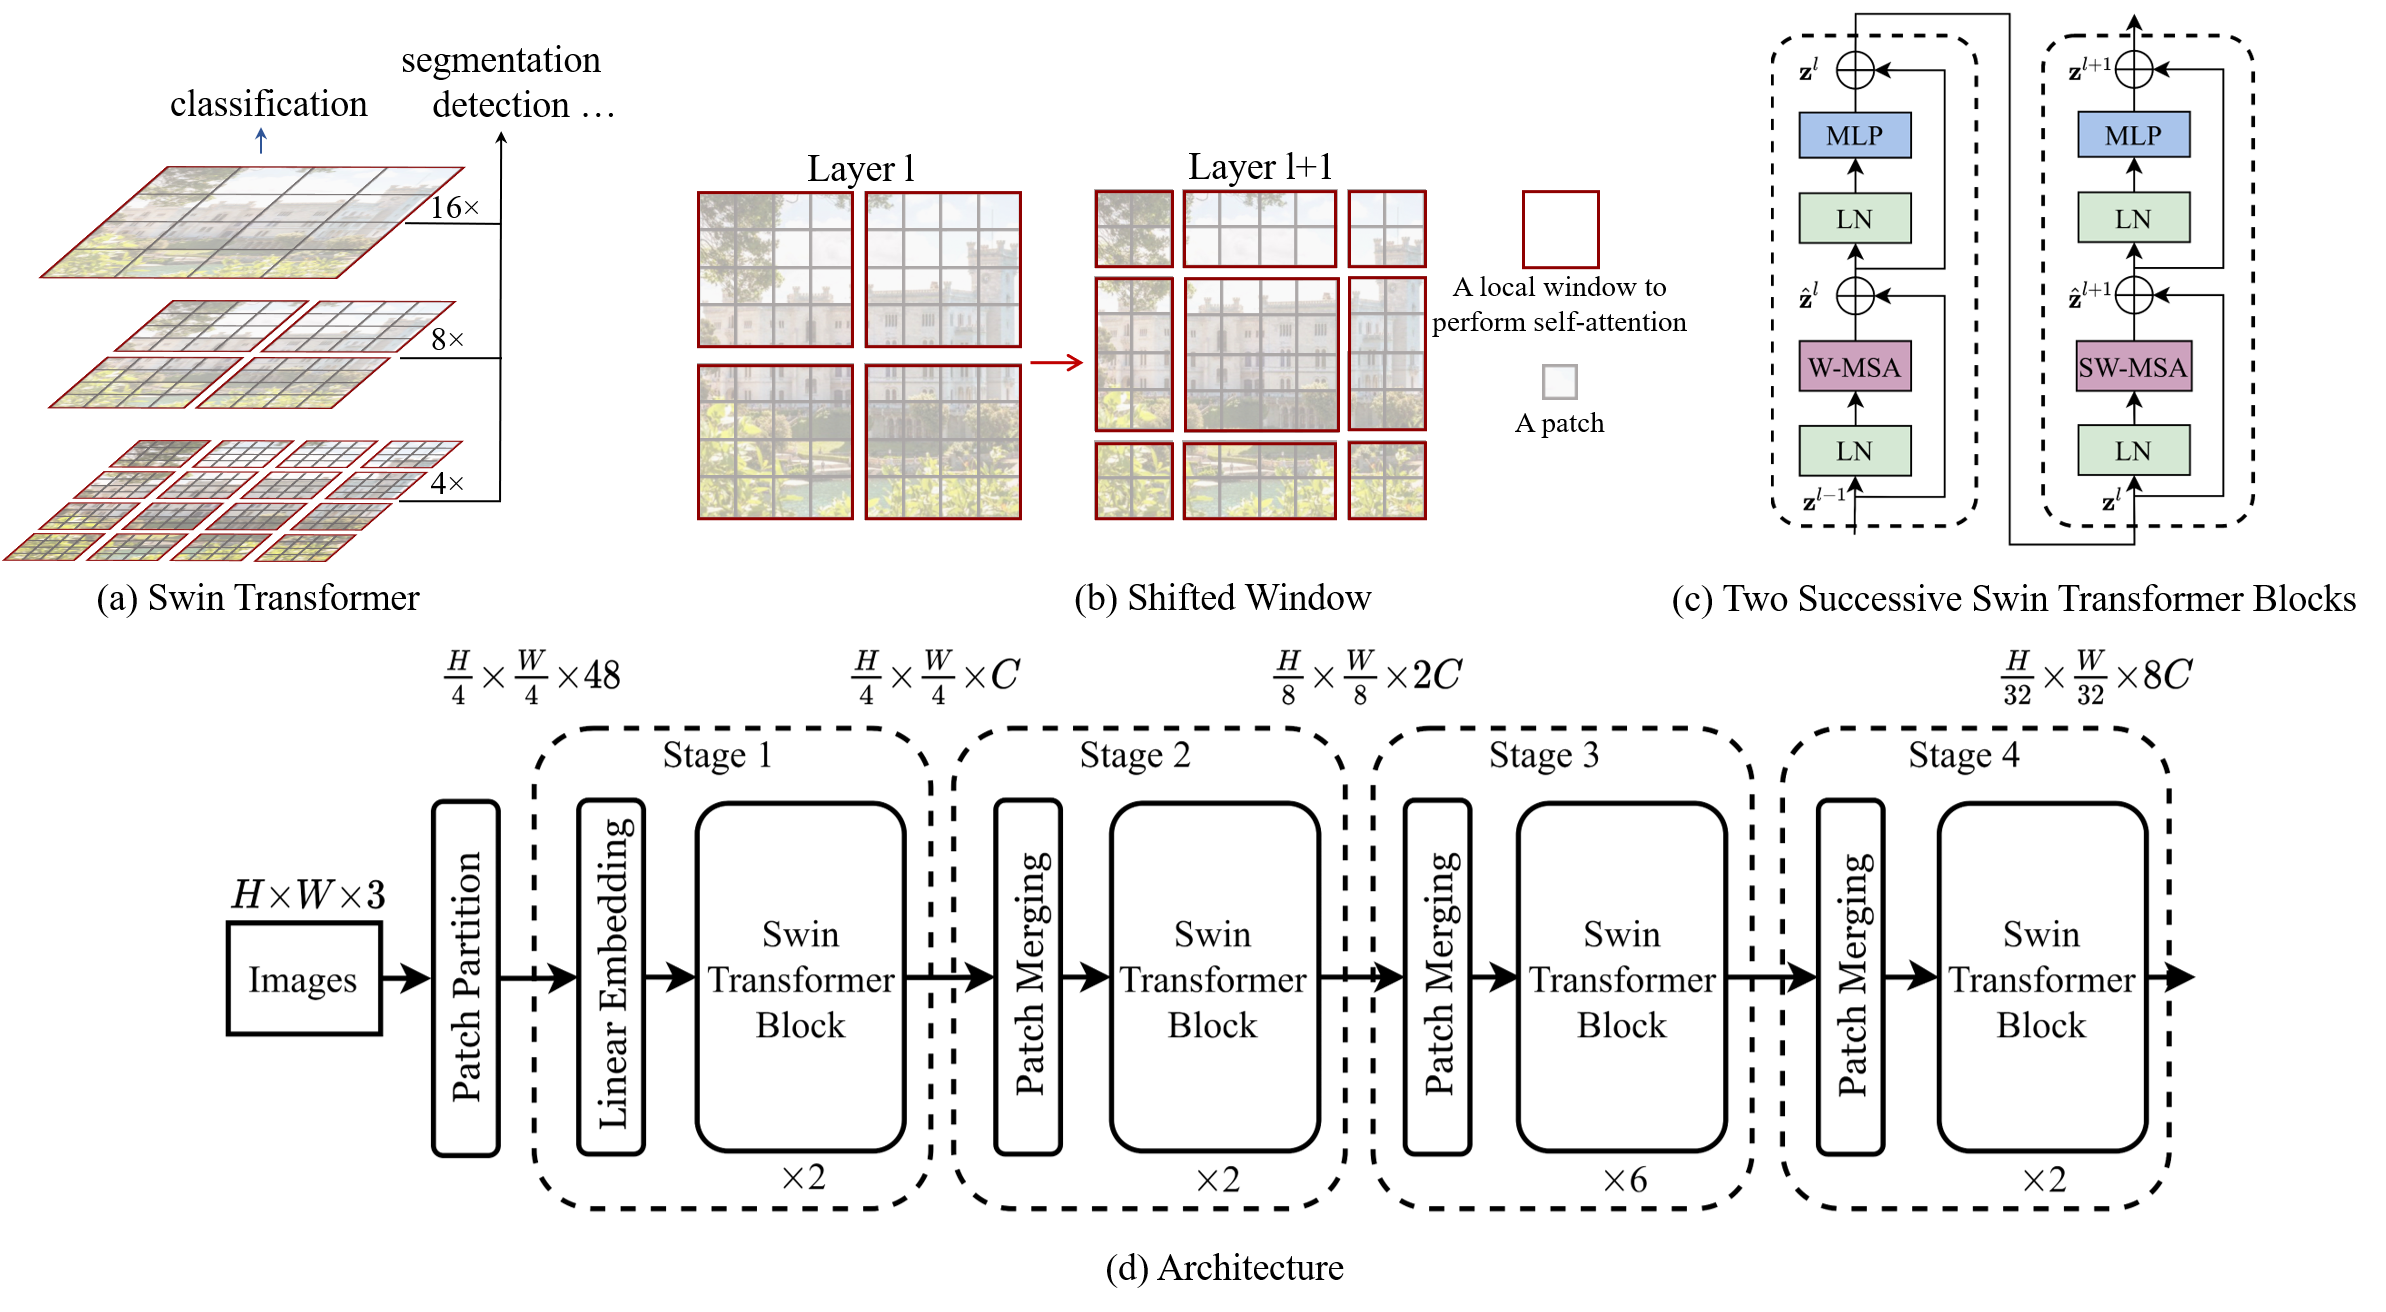
\includegraphics[width=\columnwidth]{Imagens/arquitetura swin.png}
    \caption{Arquitetura swin ~\cite{liu2022swin}}
    \label{fig:SWIN-arquitetura}
\end{figure}



\subsection{ForestViT Modelo de classificação de desmatamento}\label{sec:Cap2_ForestViT}

Em~\cite{9701667} foi proposto um classificador multiclasses baseado na arquitetura de \textit{transformers} visual. Os resultados também foram comparados com modelos baseados em CNN estabelecidos, como Resnet e VGG. 


%We utilize a dataset (URL: https://www.kaggle.com/c/planet-understanding-the-amazon-from-space/data) published in a Kaggle competition (by Planet company), containing coarse-resolution imagery data from satellites with varying spatial resolution characteristics, i.e., the imagery has a ground-sample distance (GSD) of 3.7 m and an orthorectified pixel size of 3 m. The data comes from Planet’s Flock tow satellites in both Sun-synchronous and ISS orbits and was collected in the time interval between January 1, 2016, and February 1, 2017. All of the images are derived from the Amazon basin. Mangrove deforestation in the Amazon forest is an intense phenomenon, and a plethora of factors that contribute to deforestation is observed there. Each entry contains imagery data in RGB plus the infrared band in geo-referenced.tiff format. In our experiment, the images are classified into 14 classes and the labels are broken into three groups: atmospheric conditions, common land cover/land use phenomena, and rare land cover/land use phenomena (see Fig. 3). Here, each entry is assigned to one or more classes.


% Abstract: Monitoring changes within the land surface and open water bodies is critical for natural resource management, conservation, and environmental policy. While the use of satellite imagery for these purposes is common, fine-scale change detection can be a technical challenge. Difficulties arise from variable atmospheric conditions and the problem of assigning pixels to individual objects. We examined the degree to which two machine learning approaches can better characterize change detection in the context of a current conservation challenge, artisanal small-scale gold mining (ASGM). We obtained Sentinel-2 imagery and consulted with domain experts to construct an open-source labeled land-cover change dataset. The focus of this dataset is the Madre de Dios (MDD) region in Peru, a hotspot of ASGM activity. We also generated datasets of active ASGM areas in other countries (Venezuela, Indonesia, and Myanmar) for out-of-sample testing. With these labeled data, we utilized a supervised (E-ReCNN) and semi-supervised (SVM-STV) approach to study binary and multi-class change within mining ponds in the MDD region. Additionally, we tested how the inclusion of multiple channels, histogram matching, and La*b* color metrics improved performance of the models and reduced the influence of atmospheric effects. Empirical results show that the supervised E-ReCNN method on 6-Channel histogram-matched images generated the most accurate detection of change not only in the focal region (Kappa: 0,92(±0.04), Jaccard: 0,88(±0.07), F1:0.88(±0.05)) but also in the out-of-sample prediction regions (Kappa: 0,90(±0.03), Jaccard: 0,84(±0.04), and F1: 0,77(±0.04)). While semi-supervised methods did not perform as accurately on 6- or 10-channel imagery, histogram matching and the inclusion of La*b* metrics generated accurate results with low memory and resource costs. These results show that E-ReCNN is capable of accurately detecting specific and object-oriented environmental changes related to ASGM. E-ReCNN is scalable to areas outside the focal area and is a method of change detection that can be extended to other forms of land-use modification.



% In this work we present BrazilDAM, a novel public dataset based on Sentinel-2 and Landsat-8 satellite images covering all tailings dams cataloged by the Brazilian National Mining Agency (ANM). The dataset was built using georeferenced images from 769 dams, recorded between 2016 and 2019. The time series were processed in order to produce cloud free images. The dams contain mining waste from different ore categories and have highly varying shapes, areas and volumes, making BrazilDAM particularly interesting and challenging to be used in machine learning benchmarks. The original catalog contains, besides the dam coordinates, information about: the main ore, constructive method, risk category, and associated potential damage. To evaluate BrazilDAM's predictive potential we performed classification essays using state-of-the-art deep Convolutional Neural Network (CNNs). In the experiments, we achieved an average classification accuracy of 94.11% in tailing dam binary classification task. In addition, others four setups of experiments were made using the complementary information from the original catalog, exhaustively exploiting the capacity of the proposed dataset. 


% https://huggingface.co/docs/transformers/model_doc/vit
% https://huggingface.co/blog/fine-tune-vit 
% https://huggingface.co/blog/your-first-ml-project
% https://huggingface.co/blog/accelerate-deepspeed
% https://huggingface.co/blog/fine-tune-vit